\documentclass{beamer}

% theme definition
\usetheme{KU}

\usepackage{alltt}

\setbeamertemplate{blocks}[rounded][shadow=true]

\setbeamercolor{title}{fg=kublue}
\setbeamercolor{subtitle}{fg=kugray} 
\setbeamercolor{institute}{fg=kugray}
\setbeamercolor{frametitle}{fg=kublue}
\setbeamercolor{frametitle}{bg=white}
\setbeamercolor{framesubtitle}{fg=kugray}
\setbeamercolor{framesubtitle}{bg=white}
\setbeamercolor{item}{fg=black}
\setbeamercolor{subitem}{fg=kugray}
\setbeamercolor{itemize/enumerate subbody}{fg=kugray}
\setbeamercolor{block title}{bg=kublue}
\setbeamercolor{block title}{fg=white}
\setbeamercolor{block body}{bg=sand}
\setbeamercolor{block body}{fg=black}

\usefonttheme{serif}

\newenvironment{fnverbatim}{\begin{alltt}\scriptsize}{\normalsize\end{alltt}}
\newcommand{\mean}[1]{\langle#1\rangle}
\newcommand{\rtime}{\ensuremath{\mathbb{R}^{0\leq}}}

\title{Transition Systems and Invariants}
\subtitle{EECS 755---Software Systems Modeling}

\author{Dr. Perry Alexander}

%\date{{\color{kugray}\today}}
\date{\ }

% turns off navigation symbols
\setbeamertemplate{navigation symbols}{}

\institute{
    Information and Telecommunication Technology Center \\
    Electrical Engineering and Computer Science \\
    The University of Kansas \\
    \texttt{palexand@ku.edu}}

\begin{document}

\begin{frame}
  \titlepage

%%{\footnotesize\color{kugray} Formatted with the Beamer Class for \LaTeXe}
\end{frame}

\frame{\frametitle{Presentation Outline}
  \begin{itemize}
    \item Review access control modeling objectives
      \begin{itemize}
      \item modeling platform MAC
      \item modeling local access control
      \end{itemize}
    \item Overview access control policy definition
      \begin{itemize}
      \item design and modeling assumptions
      \item platform boot policy definition
      \item local policy definitions
      \end{itemize}
    \item Overview models
      \begin{itemize}
      \item domain and system models
      \item communication model
      \item theorems and status
      \end{itemize}
    \item Identify next steps
      \begin{itemize}
      \item runtime and moving beyond the SVP line
      \item adding M\&A detail
      \end{itemize}
  \end{itemize}
}

\frame{\frametitle{Access Control Modeling Objectives}
  \framesubtitle{What we're about here}

  Reporting joint work with Geoffrey Brown, Indiana University (submitted) in which
  we verify two physical layer protocols.
  \begin{itemize}
    \item Biphase Mark Protocol (BMP)
    \item 8N1 Protocol
  \end{itemize}

These protocols are used in data transmission for CDs, Ethernet, and Tokenring,
      etc. as well as UARTs.  
  \begin{itemize}
    \item Correctness is reasonably difficult to prove due to many real-time constraints.

    \item Many previous formal modeling/verification efforts for these protocols.
  \end{itemize}

}

\frame{\frametitle{Columns and Blocks}\framesubtitle{Trying figures
    next to lists}
  \begin{columns}[c]
    \column{.45\textwidth}
%    \begin{block}{Things}
    Some normal text goes here just for introduction
    \begin{itemize}
      \item Appraisal
      \item Measurement
      \item Attestation
      \item vTPM
    \end{itemize}
    \alert{Why is this column getting higher?}\\
    Maybe it's not\\
    Center alignment seems best.\\
    \alert{I like this for two column test and graphics}\\
    Getting higher???
%    \end{block}
    \column{.45\textwidth}
    \begin{figure}
      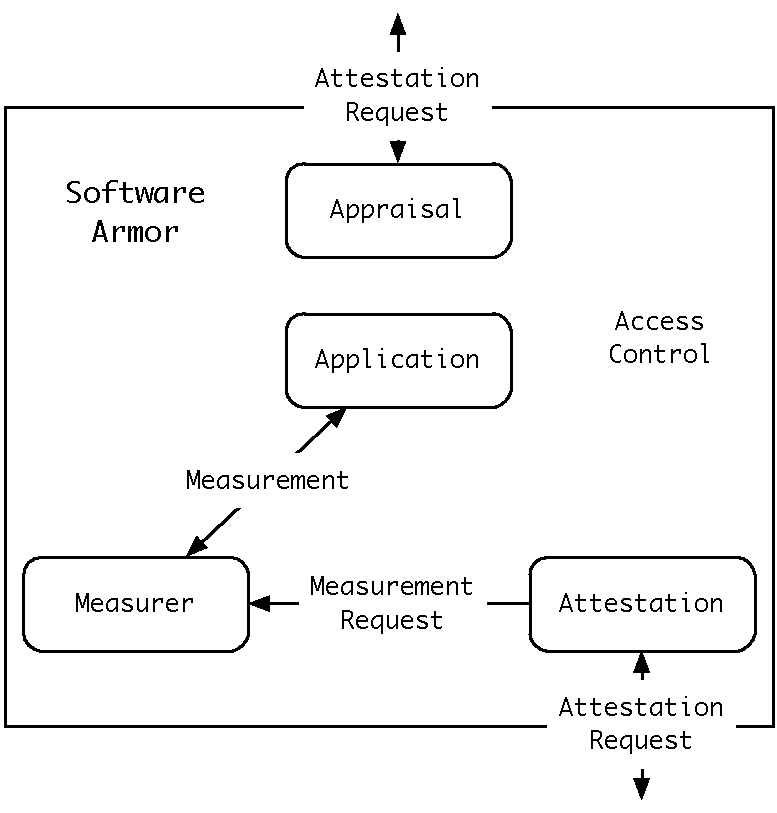
\includegraphics[width=0.95\textwidth]{architecture.pdf}
    \end{figure}
  \end{columns}
}

\frame[plain]{\frametitle{Big Picture}\framesubtitle{Armor Architecture}
  \begin{figure}
    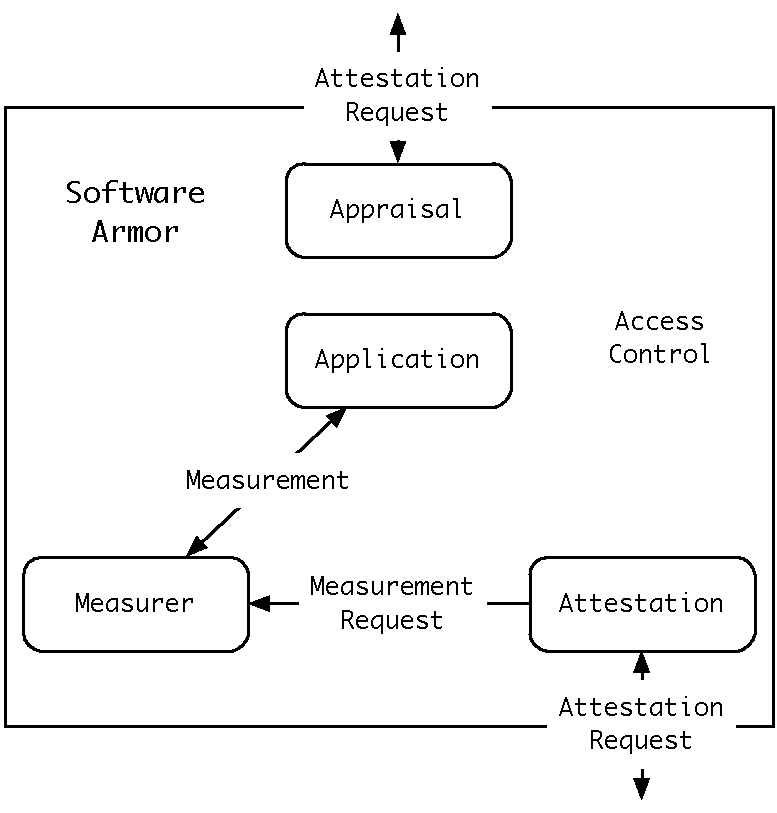
\includegraphics[height=0.70\textheight]{architecture.pdf}
  \end{figure}
}
    

{\frame{\frametitle{Simple Block}
  \begin{block}{Introduction to {\LaTeX}}
    ‘‘Beamer is a {\LaTeX}class for creating presentations
    that are held using a projector..."
  \end{block}
  
  \begin{block}{}
    This is a definition
  \end{block}
}

\frame{\frametitle{Proofs}
  \begin{proof}[Not really a proof]
    \begin{enumerate}
    \item<1-3>{This is a step}
    \item<2-3>{This is another step}
    \item<3>{This is a third step}
    \item<3>{This is a third step}
    \item<3>{This is a third step}
    \item<3>{This is a third step}
    \end{enumerate}
  \end{proof}
}


\frame{\frametitle{List with Overlays}
  \begin{itemize}
  \item<1-> Item 1 followed by a pause
  \item<3-> Item 2 followed by a pause
  \item<2-> Item 3 followed by a pause
  \end{itemize}
}

\frame{\frametitle{Previous Efforts}

  \begin{itemize}
  \item BMP has been verified in PVS twice and required
    \begin{itemize}
    \item  37 invariants and 4000 individual proof directives (initially) in the
      one effort
    \item 5 hours just to \emph{check} the proofs in the other effort
    \item A formal specification and verification of an independent real-time model
      in both efforts
    \end{itemize}
  \item BMP has been verified in (the precursor to) ACL2 by J. Moore and required
    \begin{itemize}
     \item A significant conceptual effort to fit the problem in the logic, arguably
       omitting some salient features of the model
     \item The statement and proof of many antecedent results
     \item J. Moore reports this as one of his ``best ideas'' in his career
    \end{itemize}
    
  \end{itemize}
}

\frame{\frametitle{Not Your Father's Theorem-Prover} 

The verifications are carried out in the SAL infinite-state bounded model-checker
that combines SAT-solving and SMT decision procedures to \emph{prove} safety
properties about infinite-state models.

  \begin{itemize}
    \item Theorem-proving efforts took multiple engineer-months if not years to
      complete.

    \item Our initial effort in SAL consumed about \emph{two engineer-days}.\\
      ...and we found a significant bug in a UART application note.
  \end{itemize}
}


\frame[containsverbatim]{\frametitle{Parameterized Timing Constraints}
SMT allows for {\color{red}\emph{parameterized}} proofs of correctness.  The following are
example constaints from the BMP verification:
\begin{fnverbatim}
  TIME: TYPE = REAL;

  TPERIOD: TIME = 16;
  TSAMPLE: INTEGER = 23;
{\color{red}
  TSETTLE}: \{x: TIME |     0 <= x  
                      AND (x + TPERIOD < TSAMPLE) 
                      AND (x + TSAMPLE + 1 < 2 * TPERIOD)\};
{\color{red}
  TSTABLE}: TIME = TPERIOD - TSETTLE;
{\color{red}  
  ERROR}: \{x: TIME |     (0 <= x) 
                    AND (TPERIOD + TSETTLE < TSAMPLE*(1-x)) 
                    AND (TSAMPLE*(1+x) + (1+x) + TSETTLE < 2 * TPERIOD)\};

  RSAMPMAX: TIME = TSAMPLE * (1 + ERROR);
  RSAMPMIN: TIME = TSAMPLE * (1 - ERROR);
  RSCANMAX: TIME = 1 + ERROR;
  RSCANMIN: TIME = 1 - ERROR;
\end{fnverbatim}
}


\frame[containsverbatim]{\frametitle{SRI's SAL Toolset}
      \begin{itemize}
        \item Parser
        \item Simulator
        \item Symbolic model-checker (BDDs) 
        \item Witness symbolic model-checker 
        \item Bounded model-checker
        \item Infinite-state bounded model-checker
        \item Future releases include: 
          \begin{itemize}
            \item Explicit-state model-checker
            \item MDD-based symbolic model-checking
          \end{itemize}
      \end{itemize}
\begin{center}
All of which are ``state-of-the-art''
\end{center}
}


\frame{\frametitle{$k$-Induction}

Please direct your attention to the whiteboard.

}



\frame[label=ta]{ \frametitle{Timeout Automata\footnote{B. Dutertre
  and M. Sorea.  Timed systems in SAL.  \emph{SRI TR}, 2004.} (Semantics)}

  An \emph{explicit} real-time model.

  \begin{itemize}
  \item Vocabulary:
  \begin{itemize}
    \item A set of state variables.
    \item A \emph{global clock}, $c \in \rtime$.
    \item A set of \emph{timeout} variables $T$ such that for $t \in
      T$, $t \in \rtime$.
  \end{itemize}
  \item Construct a transition system $\mean{S, \, S^0, \, \rightarrow}$:
  \begin{itemize}
    \item States are mappings of all variables to values.
    \item Transitions are either \emph{time transitions} or
      \emph{discrete transitions}.
      \begin{itemize}
        \item Time transitions are enabled if the clock is less than
          all timeouts.  Updates clock to least timeout.
        \item Discrete transitions are enabled if the clock equals
          some timeout.  Updates state variables and timeouts.
      \end{itemize}
  \end{itemize}
  \end{itemize}
}

\frame[containsverbatim]{\frametitle{Disjunctive Invariants} Even with $k$-induction, getting a
  sufficiently strong invariant is still hard!  \emph{Disjunctive invariants} help.
  A disjunctive invariant can be built iteratively from the counterexamples returned
  for the hypothesized invariant being verified.

\begin{fnverbatim}
  t0:  THEOREM system |- 
         G(   (    (phase = Settle) 
               AND (rstate = tstate + 1) 
               AND (rclk - tclk - TPERIOD > 0) 
               AND (tclk + TPERIOD + TSTABLE - rclk > 0))
           OR
              (    (phase = Stable) 
               AND (rstate = tstate + 1) 
               AND (rclk - tclk - TSETTLE > 0) 
               AND (tclk + TPERIOD - rclk > 0)  
               AND (rdata = tdata))

                        .
                        .
                        .
\end{fnverbatim}
}


\end{document}

